\documentclass{beamer}

\usetheme{Warsaw}
\usecolortheme{default}

\usepackage[MeX]{polski}
\usepackage[cp1250]{inputenc}
\usepackage{graphicx}

\setbeamercovered{dynamic}

\title{IIviewer}
\author{Konrad Garlikowski, Dawid Jasi�ski}
\date{\today}

\begin{document}

\frame{\titlepage}

\section[Spis]{}
\frame{
	\tableofcontents
}

\section{Szczeg�y}

\subsection{Warstwy}
\frame
{
  \frametitle{Warstwy}

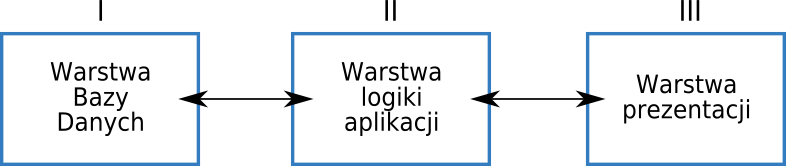
\includegraphics[width=300pt, height=60pt]{warstwy}

\begin{itemize}
  	\item I - warstwa Bazy Danych
  	Dzieli sie na 2 odrebne elementy:
    	\begin{itemize}
  			\item Faktycznia Baze Danych "`SQLite"', kt�ra b�dzie magazynem informacji dotycz�cych zdj�� u�ytkownika
  			\item System plikow, kt�ry b�dzie s�u�y� do przechowywania wygenerowanych miniaturek 
  		\end{itemize}
  		
  	\item II - warstwa logiki aplikacji. W tej warstwie b�d� odbywa�y sie wszystkie transformacje zdj�c, odczyt/zapis. B�dzie po�rednikiem miedzy warstwa I, a III
  	   \begin{itemize}
  			\item Cos
  		 \end{itemize}  

     	\item III - warstwa prezentacji
  	B�dzie ona stanowi�a �atwe w obs�udze GUI. W jej sk�ad b�d� wchodzi�y:
  	   \begin{itemize}
  			\item R�ne widoki obrazk�w
  			\item Elementy nawigacyjne
  			\item Inne 
  		 \end{itemize}  
   \end{itemize}

}

\end{document}